\documentclass[../DoAn.tex]{subfiles}
\begin{document}
Từ những vấn đề thực tế cùng với tổng quan về đề tài được đề cập trong Chương 1, Chương 2 sẽ đi sâu hơn về một số sản phẩm liên quan hiện nay và phân tích chi tiết yêu cầu của hệ thống quản lý dữ liệu hiển thị trong mục 2.2.

% Với phương pháp phân tích thiết kế hướng đối tượng, sinh viên sử dụng biểu đồ use case theo hướng dẫn của template này. Với các phương pháp khác, sinh viên trao đổi với giáo viên hướng dẫn để đổi tên và 

% \textbf{Lưu ý}: Mỗi chương nên có thêm 1 đoạn mở đầu chương và kết thúc chương, mở đầu giới thiệu những nội dung sẽ trình bày trong chương, kết thúc tổng kết lại các nội dung đã trình bày

\section{Khảo sát hiện trạng}
\label{section:2.1}
% Hiện nay, có rất nhiều cách cho các doanh nghiệp để quản lý 
% Thông thường, khảo sát chi tiết về hiện trạng và yêu cầu của phần mềm sẽ được lấy từ ba nguồn chính, đó là (i) người dùng/khách hàng, (ii) các hệ thống đã có, (iii) và các ứng dụng tương tự.
% Sinh viên cần tiến hành phân tích, so sánh, đánh giá chi tiết ưu nhược điểm của các sản phẩm/nghiên cứu hiện có. Sinh viên có thể lập bảng so sánh nếu cần thiết. Kết hợp với khảo sát người dùng/khách hàng (nếu có), sinh viên nêu và mô tả sơ lược các tính năng phần mềm quan trọng cần phát triển.

\section{Tổng quan chức năng}
\label{section:2.2}
% Phần \ref{section:2.2} này có nhiệm vụ tóm tắt các chức năng của phần mềm. Trong phần này, sinh viên lưu ý chỉ mô tả chức năng mức cao (tổng quan) mà không đặc tả chi tiết cho từng chức năng. Đặc tả chi tiết được trình bày trong phần \ref{section:2.3}.

\subsection{Biểu đồ use case tổng quát}
\label{subsection:2.2.1}
% Sinh viên vẽ biểu đồ use case tổng quan và giải thích các tác nhân tham gia là gì, nêu vai trò của từng tác nhân, và mô tả ngắn gọn các use case chính.

Hình 1 dưới đây là biểu đồ use case tổng quan của hệ thống quản lý thông tin và thiết bị EPD. Có 3 tác nhân chính tham gia hệ thống, bao gồm (i) Người quản lý, Quản trị viên và các thiết bị EPD. Người quản lý có thể quản lý các thiết bị EPD, các nội dung thông tin và quản lý tài khoản cá nhân của mình. Quản trị viên được kế thừa các chức năng của Người quản lý và cũng có thể quản lý kiểm thử các thiết bị sâu hơn. Các thiết bị tham gia hệ thống đóng vai trò là thiết bị đầu cuối, nhận và hiển thị dữ liệu trên màn hình, cũng như giao tiếp với hệ thống qua giao thức MQTT.
\begin{figure}[h]
    \centering
    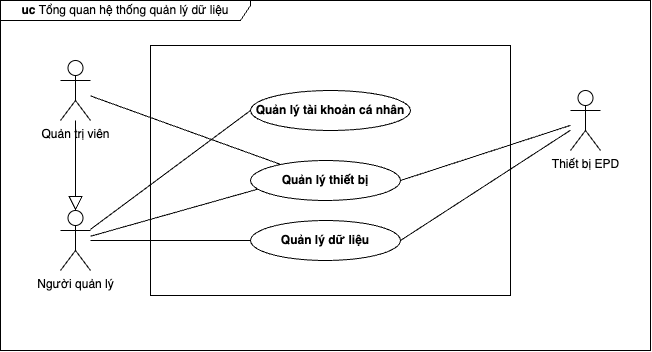
\includegraphics[scale=0.6]{imgs/diagrams/uc_general.png}
    \caption{Biểu đồ use-case tổng quan hệ thống quản lý dữ liệu.}
    \label{fig:uc-general}
\end{figure}


\subsection{Biểu đồ use case phân rã}
\label{subsection:2.2.2}
\subsubsection{Biểu đồ use case phân rã quản lý tài khoản cá nhân người dùng}

Hình 2 là biểu đồ use case phân rã chức năng quản lý tài khoản cá nhân của người dùng, bao gồm Người quản lý và Quản trị viên. Người dùng có thể tạo tài khoản, đăng nhập và chỉnh sửa thông tin cá nhân của mình.
\begin{figure}[h]
    \centering
    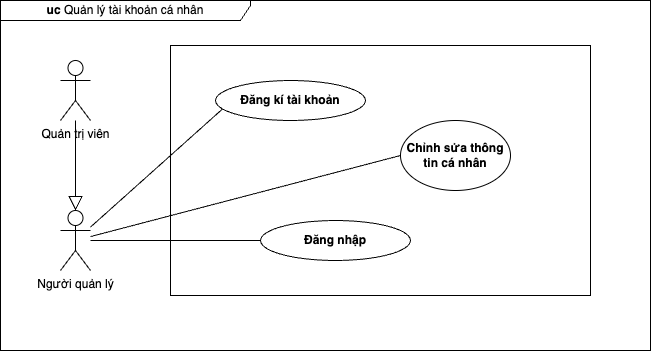
\includegraphics[scale=0.6]{imgs/diagrams/uc_account.png}
    \caption{Biểu đồ use case phân rã quản lý tài khoản cá nhân người dùng.}
    \label{fig:uc-general}
\end{figure}

% Với mỗi use case mức cao trong biểu đồ use case tổng quan, sinh viên tạo một mục riêng như mục \ref{subsection:2.2.2} và tiến hành phân rã use case đó. Lưu ý tên use case cần phân rã trong biểu đồ use case tổng quan phải khớp với tên đề mục.

% Trong mỗi mục như vậy, sinh viên vẽ và giải thích ngắn gọn các use case phân rã.
\subsubsection{Biểu đồ use case phân rã quản lý dữ liệu}

Hình 3 là biểu đồ use case phân rã chức năng quản lý dữ liệu của Người quản lý. Người quản lý có thể xem danh sách, thêm, chỉnh sửa hoặc xóa thông tin dữ liệu, hoặc cũng có thể lựa chọn hiển thị trên thiết bị hay không. 
\begin{figure}[h]
    \centering
    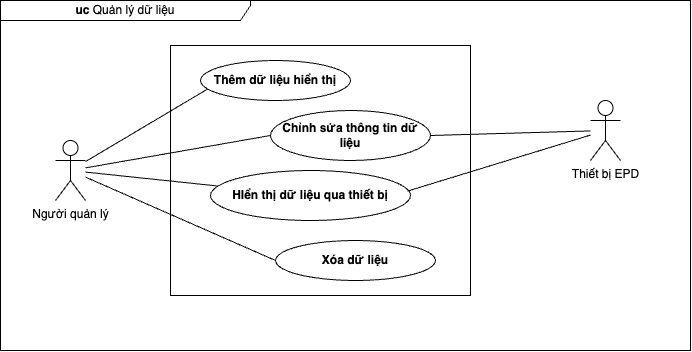
\includegraphics[scale=0.6]{imgs/diagrams/uc_data.png}
    \caption{Biểu đồ use case phân rã quản lý dữ liệu.}
    \label{fig:uc-general}
\end{figure}

\subsubsection{Biểu đồ use case phân rã quản lý thiết bị}

Hình 4 là biểu đồ use case phân rã chức năng quản lý thiết bị của Người quản lý và Quản trị viên. Người quản lý có thể đăng kí thiết bị vào hệ thống, chỉnh sửa thông tin thiết bị hoặc xóa thiết bị khỏi hệ thống. Quản trị viên, với kế thừa các chức năng của Người quản lý, ngoài ra có thể kiểm thử thiết bị khi kết nối với máy tính qua USB.
\begin{figure}[h]
    \centering
    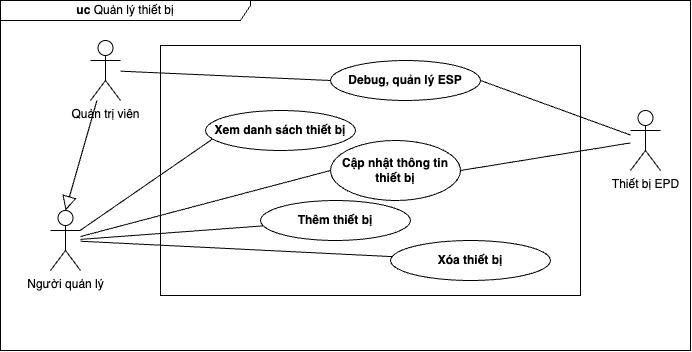
\includegraphics[scale=0.6]{imgs/diagrams/uc_device.png}
    \caption{Biểu đồ use case phân rã quản lý thiết bị.}
    \label{fig:uc-general}
\end{figure}

\subsection{Quy trình nghiệp vụ}
\label{subsection:2.2.3}
Trong hệ thống quản lý dữ liệu có nhiều quy trình nghiệp vụ, nổi bật nhất là quy trình thêm dữ liệu và hiển thị trên thiết bị EPD, và quy trình thêm thiết bị EPD vào hệ thống. Mỗi quy trình đều thể hiện quá trình hệ thống giao tiếp với thiết bị qua cổng USB và giao thức MQTT, và cách thiết bị nhận và xử lý dữ liệu.
\subsubsection{Quy trình tạo thiết bị mới}
Hình 5 dưới đây mô tả quy trình nghiệp vụ khi Người quản lý tạo và đăng kí thiết bị mới trên hệ thống. Quy trình này yêu cầu người dùng kết nối thiết bị EPD với máy tính qua cổng USB, sau đó chọn thiết bị đã kết nối trên hệ thống, điền thông tin và sau đó gửi lên hệ thống. Khi hệ thống nhận được yêu cầu đăng kí thiết bị mới, nó cũng sẽ gửi yêu cầu ghi thông tin vào thiết bị đang kết nối qua giao thức Serial Port. Khi nhận được thông tin được gửi qua, thiết bị EPD sẽ kết nối với Internet và kết nối với MQTT Broker, và gửi lại thông tin trạng thái đến hệ thống.
\begin{figure}[h]
    \centering
    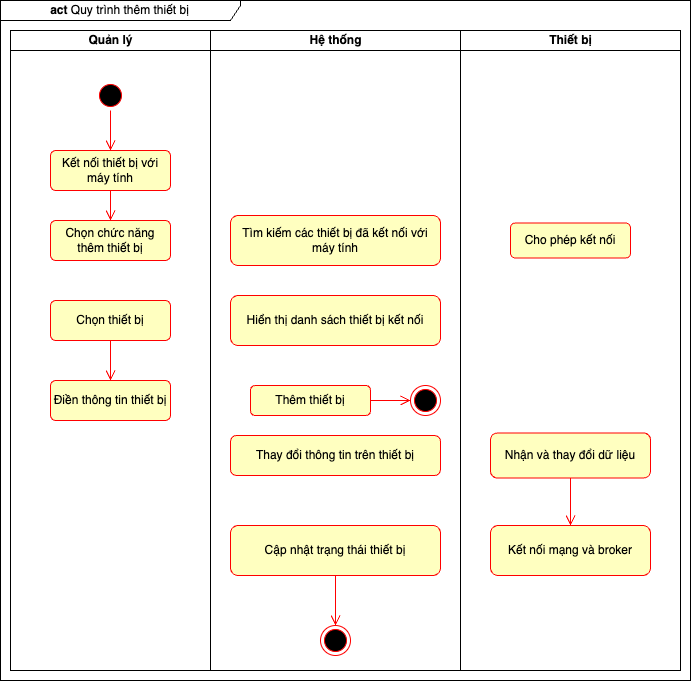
\includegraphics[scale=0.6]{imgs/diagrams/act_addDevice.png}
    \caption{Quy trình tạo thiết bị mới.}
    \label{fig:uc-general}
\end{figure}
\subsubsection{Quy trình tạo dữ liệu và hiển thị trên thiết bị}
Hình 6 dưới đây mô tả quy trình nghiệp vụ khi người dùng thêm dữ liệu vào hệ thống. Đầu tiên, người dùng sẽ chọn loại dữ liệu muốn hiển thị, sau đó dựa vào loại dữ liệu đã chọn trên, người dùng thêm thông tin chi tiết tương ứng. Người dùng cũng có thể lựa chọn cho phép hiển thị trên thiết bị EPD hay không. Nếu cho phép, hệ thống sẽ lấy lấy danh sách các thiết bị đang kết nối với MQTT Server để người dùng lựa chọn, và người dùng sẽ điền thêm thông tin về cách hiển thị trên thiết bị. Sau khi nhận được thông tin từ người dùng, hệ thống sẽ gửi thông điệp MQTT qua MQTT Broker, và thiết bị được lựa chọn sẽ nhận và hiển thị thông tin và gửi lại trạng thái đến hệ thống qua giao thức MQTT.

\begin{figure}[h]
    \centering
    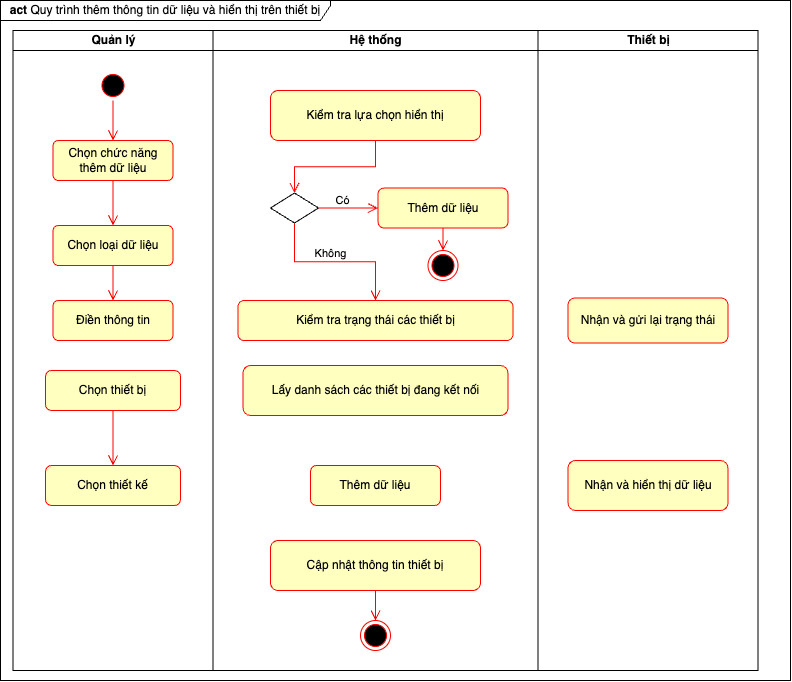
\includegraphics[scale=0.6]{imgs/diagrams/act_addData.png}
    \caption{Quy trình tạo dữ liệu và hiển thị trên thiết bị.}
    \label{fig:uc-general}
\end{figure}

\section{Đặc tả chức năng}
\label{section:2.3}
Sinh viên lựa chọn từ 4 đến 7 use case quan trọng nhất của đồ án để đặc tả chi tiết. Mỗi đặc tả bao gồm ít nhất các thông tin sau: (i) Tên use case, (ii) Luồng sự kiện (chính và phát sinh), (iii) Tiền điều kiện, và (iv) Hậu điều kiện. Sinh viên chỉ vẽ bổ sung biểu đồ hoạt động khi đặc tả use case phức tạp.
\subsection{Đặc tả use case A}

\begin{longtable}{|l|l|l|p{6cm}|}
    \hline
    \textbf{Mã use case} & UC01 & \textbf{Tên use case} & Quản lý thiết bị \\ \hline

    \textbf{Tác nhân} & \multicolumn{3}{l|}{Người quản lý} \\ \hline

    \textbf{Tiền điều kiện} & \multicolumn{3}{p{12cm}|}{Người dùng đăng nhập vào hệ thống với vai trò là Người quản lý. Với nghiệp vụ tạo thiết bị mới và chỉnh sửa thông tin thiết bị trong trường hợp thiết bị không kết nối tới Internet, người dùng cần phải kết nối thiết bị với máy tính qua cổng USB.} \\ \hline

% \multirow{8}{*}{\rotatebox[origin=c]{90}{Luồng sự kiện chính (thành công)}} & STT & Thực hiện bởi & Hành động \\ \cline{2-4}
% & 1 & Người quản lý & Chọn chức năng thêm thiết bị \\ \cline{2-4}
% & 2 & Hệ thống & Lấy và hiển thị danh sách các thiết bị đang kết nối qua USB. \\ \cline{2-4}
% & ... & ... & ... \\ \cline{2-4}
% & ... & ... & ... \\ \cline{2-4}
% & ... & ... & ... \\ \cline{2-4}
% & ... & ... & ... \\ \cline{2-4}
% & ... & ... & ... \\ \hline

    \multicolumn{4}{|l|}{a)	Thêm thiết bị mới} \\ 
    \multicolumn{4}{|l|}{
        \begin{tabular}{|p{2cm}|c|c|p{6cm}|}
            \hline
            \multirow{12}{}{\textbf{Luồng sự kiện chính (thành công)}} & 
            \textbf{STT} & \textbf{Thực hiện bởi} & \textbf{Hành động} \\ \cline{2-4}
            & 1     & Người quản lý             & Chọn chức năng thêm thiết bị \\ \cline{2-4}
            & 2     & Hệ thống                  & Lấy và hiển thị danh sách các thiết bị đang kết nối qua USB \\ \cline{2-4}
            & 3     & Người quản lý             & Lựa chọn thiết bị từ danh sách \\ \cline{2-4}
            & 4	    & Hệ thống                  & Kết nối với thiết bị qua cổng Serial Port \\ \cline{2-4}
            & 5	    & Hệ thống	                & Hiển thị giao diện điền thông tin thiết bị \\ \cline{2-4}
            & 6     & Người quản lý	            & Điền các thông tin của thiết bị (mô tả phía dưới *) \\ \cline{2-4}
            & 7     & Người quản lý	            & Gửi yêu cầu tạo thiết bị mới \\ \cline{2-4}
            & 8	    & Hệ thống	                & Thực hiện việc lưu dữ liệu tại server và truyền dữ liệu sang thiết bị đang kết nối \\ \cline{2-4}
            & 8.1	& Hệ thống	                & Lưu thông tin thiết bị mới tại server \\ \cline{2-4}
            & 8.2	& Hệ thống	                & Truyền dữ liệu sang thiết bị EPD \\ \cline{2-4}
            & 8.2.1	& Thiết bị EPD đang kết nối	& Xử lý thông tin nhận được \\ \cline{2-4}
            & 8.2.2	& Thiết bị EPD đang kết nối & Kết nối Internet và MQTT Broker \\ \cline{2-4}
            & 8.2.3	& Thiết bị EPD đang kết nối	& Gửi thông tin trạng thái đến server \\ \cline{2-4}
            & 8.2.4	& Hệ thống	                & Nhận và chỉnh sửa thông tin thiết bị mới \\ \cline{2-4}
            & 9	    & Hệ thống	                & Thông báo tạo thiết bị thành công \\ \hline




            \multirow{12}{}{\textbf{Luồng sự kiện thay thế}} & 
            \textbf{STT} & \textbf{Thực hiện bởi} & \textbf{Hành động} \\ \cline{2-4}
            & 4a.	 & Hệ thống	& Thông báo lỗi: không thể kết nối đến thiết bị\\ \cline{2-4}
            & 8.1a	 & Hệ thống	& Thông báo lỗi: cần nhập đủ các trường thông tin cần thiết của thiết bị nếu Người quản lý nhập thiếu\\ \cline{2-4}
            & 8.2.2a & Hệ thống	& Không nhận được phản hồi cập nhật trạng thái từ thiết bị, lưu lại thông tin thiết bị\\ \hline
        \end{tabular}
    } \\ \hline
    \multicolumn{4}{|l|}{b) Chỉnh sửa thông tin thiết bị} \\ 
    \multicolumn{4}{|l|}{
        \begin{tabular}{|p{2cm}|c|c|p{6cm}|}
            \hline
            \multirow{12}{}{\textbf{Luồng sự kiện chính (thành công)}} & 
            \textbf{STT} & \textbf{Thực hiện bởi} & \textbf{Hành động} \\ \cline{2-4}
            & 1	& Người quản lý	& Chọn chức năng thêm thiết bị \\ \cline{2-4}
            & 2	& Hệ thống	& Lấy và hiển thị danh sách các thiết bị đang kết nối qua USB. \\ \cline{2-4}
            & 3	& Người quản lý	& Lựa chọn thiết bị từ danh sách \\ \cline{2-4}
            & 4	& Hệ thống	& Kết nối với thiết bị qua cổng Serial Port \\ \cline{2-4}
            & 5	& Hệ thống	& Hiển thị giao diện điền thông tin thiết bị \\ \cline{2-4}
            & 6 	& Người quản lý	& Điền các thông tin của thiết bị (mô tả phía dưới *) \\ \cline{2-4}
            & 7	& Người quản lý	& Gửi yêu cầu tạo thiết bị mới \\ \cline{2-4}
            & 8	& Hệ thống	& Thực hiện việc lưu dữ liệu tại server và truyền dữ liệu sang thiết bị đang kết nối \\ \cline{2-4}
            & 8.1	& Hệ thống	& Lưu thông tin thiết bị mới tại server \\ \cline{2-4}
            & 8.2	& Hệ thống	& Truyền dữ liệu sang thiết bị EPD \\ \cline{2-4}
            & 8.2.1	& Thiết bị EPD đang kết nối	& Xử lý thông tin nhận được \\ \cline{2-4}
            & 8.2.2	& Thiết bị EPD đang kết nối	& Kết nối Internet và MQTT Broker \\ \cline{2-4}
            & 8.2.3	& Thiết bị EPD đang kết nối	& Gửi thông tin trạng thái đến server \\ \cline{2-4}
            & 8.2.4	& Hệ thống	& Nhận và chỉnh sửa thông tin thiết bị mới \\ \cline{2-4}
            & 9	& Hệ thống	& Thông báo tạo thiết bị thành công \\ \hline
            

            \multirow{12}{}{\textbf{Luồng sự kiện thay thế}} & 
            \textbf{STT} & \textbf{Thực hiện bởi} & \textbf{Hành động} \\ \cline{2-4}
            & 4a.	 & Hệ thống	& Thông báo lỗi: không thể kết nối đến thiết bị\\ \cline{2-4}
            & 8.1a	 & Hệ thống	& Thông báo lỗi: cần nhập đủ các trường thông tin cần thiết của thiết bị nếu Người quản lý nhập thiếu\\ \cline{2-4}
            & 8.2.2a & Hệ thống	& Không nhận được phản hồi cập nhật trạng thái từ thiết bị, lưu lại thông tin thiết bị\\ \hline

            
        \end{tabular}
    } \\ \hline
    
    \multicolumn{4}{|l|}{d) Xem danh sách thiết bị} \\ \hline

\end{longtable}


\begin{tabular}{|l|l|l|p{4cm}|}
\hline
\textbf{Mã use case} & \textbf{UC01} & \textbf{Tên use case} & \textbf{Quản lý thiết bị} \\ \hline
\textbf{Tác nhân} & \multicolumn{3}{l|}{Người quản lý} \\ \hline
\textbf{Tiền điều kiện} & \multicolumn{3}{p{9cm}|}{Người dùng đăng nhập vào hệ thống với vai trò là Người quản lý...} \\ \hline

% ... More rows as needed
\end{tabular}


\subsection{Đặc tả use case B}
\hfill

\section{Yêu cầu phi chức năng}
\label{section:2.4}
% Trong phần này, sinh viên đưa ra các yêu cầu khác nếu có, bao gồm các yêu cầu phi chức năng như hiệu năng, độ tin cậy, tính dễ dùng, tính dễ bảo trì, hoặc các yêu cầu về mặt kỹ thuật như về CSDL, công nghệ sử dụng, v.v.

Với đặc thù của hệ thống khi một người sử dụng phải quan lý rât nhiều các dữ liệu khác nhau với nhiều thiết bị trong một môi trường mở, bảo mật hệ thống là một ưu tiên hàng đầu khi giao tiếp giữa các thiết bị với nhau. Cùng với đó, hệ thống cũng yêu cầu tính minh bạch, thân thiện với người dùng mới, người dùng với khiếm khuyết cơ thể, ... Bên cạnh đó, để hoạt động ổn định trong các môi trường doanh nghiệp lớn, nhiều thiết bị, user, data, ... hệ thống cũng có nhiều yêu cầu về tính chịu đựng lỗi, dễ dàng kiểm tra, nâng cấp, bảo trì.

\subsection{Yêu cầu về bảo mật}
Về yêu cầu bảo mật, hệ thống yêu cầu các thiết bị phải giao tiếp với nhau qua TLS/SSL, bao gồm HTTPs và MQTTs.Tất cả các thiết bị trước khi kết nối đến server 
%%%%%%%%%%%%%%%%%%%%%%%%%%%%%%%%%%%

\end{document}